% ब
\section{Solution 3:  Metadata Column Family} \label{s:design-sol3}

In Solution~3,  metadata for all the column families in a keyspace is stored in a
separate column family called \texttt{Metadata}.    In this approach,  the
metadata is decoupled from the actual data and stored in a centralised way where all the
\ac{PK} and \ac{FK} constraints of all the column families within a keyspace are
saved in a single location.   The other column families contain only the actual
data and do not store any metadata.   Using this approach,   all the existing
constraints are saved as super columns in the \texttt{Metadata} column family.  
Figure~\ref{fd:Metadata-Solution3} shows an example of the \texttt{Metadata}
column family with some of the constraints of the University keyspace. 

 	 
	

The different parts of the constraints are saved as separate columns in the
\texttt{Metadata} column family.  Thus,   no special characters are required to
identify the various parts as seen in Solutions~1 and 2.   When an operation is
invoked on a column family in the keyspace referential integrity validations are
triggered.   For these validations,   it is necessary to connect to
\texttt{Metadata} column family and retrieves the relevant constraints for the
column family on which the operation is invoked. 
Thus,  the different parts of the constraints are accessed by identifying the
correct columns in the \texttt{Metadata} column family and necessary values are
retrieved to do the validation. 

This approach is similar to the way dependency information is
stored in traditional \acp{RDBMS},   where metadata holds information
about tables,   its dependencies and its many other properties.   Commonly,   such
metadata is maintained in \texttt{System} tables,  separated from the
tables containing the actual data,  as seen in this approach.   
% Such tables  cannot be altered
% directly by the users and they can only query these tables for information.  
% Such an approach keeps metadata safe and away from users thus
% avoiding any mishandling of the metadata.   

The design to decouple metadata from the actual data is inspired from the
potential challenges in Solutions~1 and 2 where
% Such cases are when metadata undergoes frequent changes or a column family has
% many constraints.  
a column family with several constraints will have a
large value in the \texttt{Metadata} column,  hence making it cumbersome to
maintain such metadata within a single string. 
Moreover,  in these solutions metadata has to be changed at every place it is repeated in the event of any alterations to
the metadata.  
Consider Solution~1,  where the \texttt{Metadata} column in every super column
of every column family has to be updated every time a constraint is added,  
removed or changed; similarly,  in Solution~2 where the top row has to be updated
for all the column families.
 
\begin{landscape}
 	\begin{figure}[c] 
		\centering
		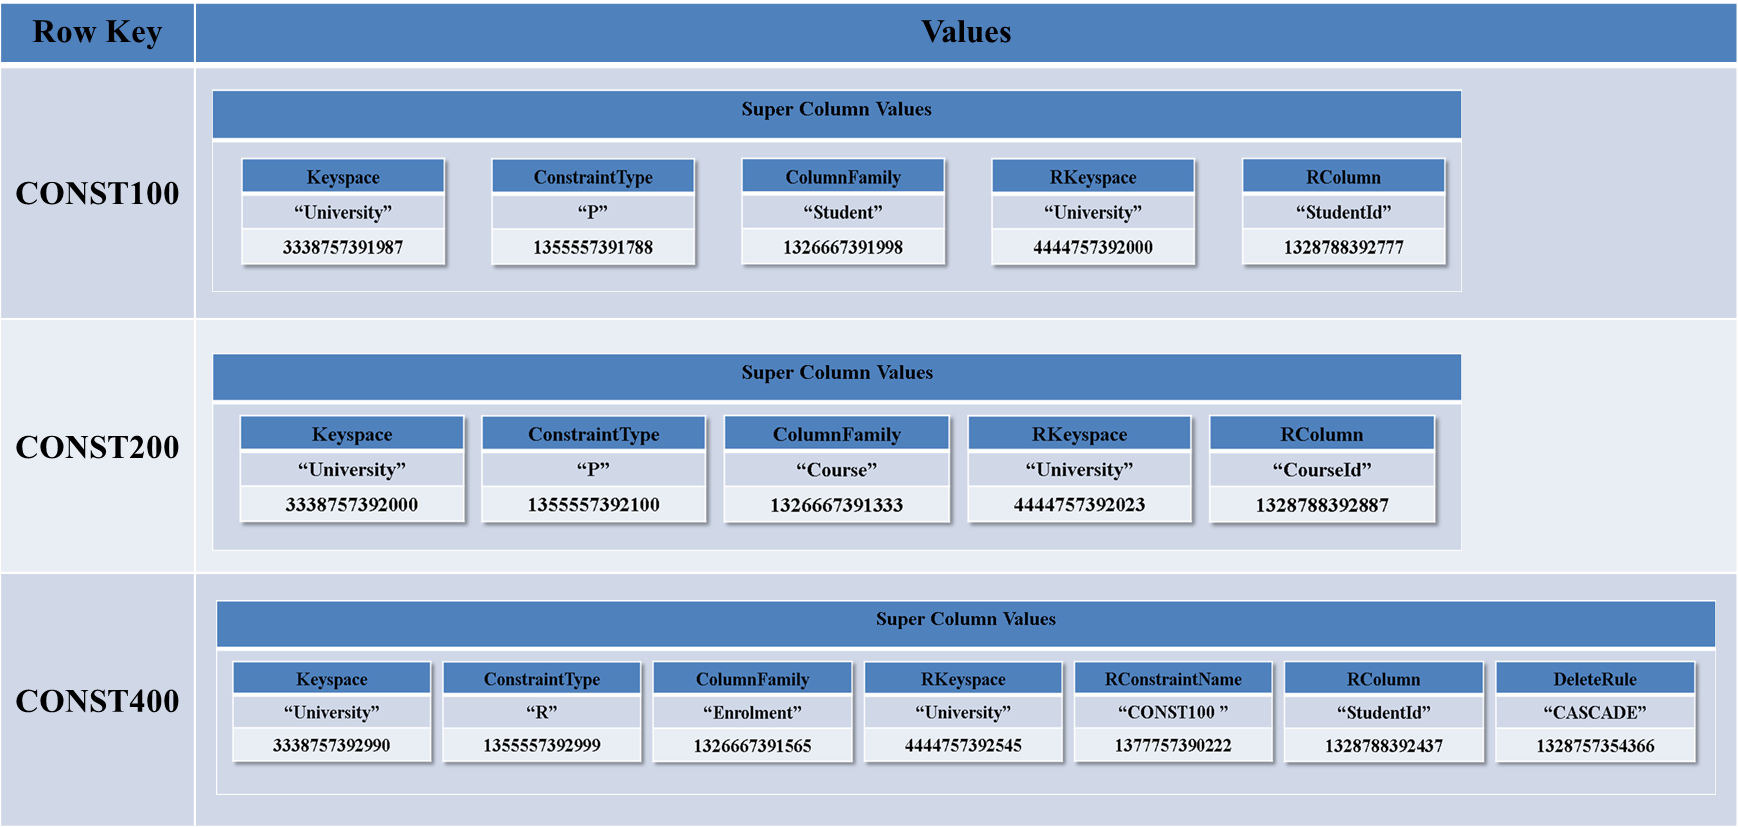
\includegraphics[width=1.45\textwidth]{./figure/Solutions/Sol3-MD-ColumnFamily.png}
		\caption{Metadata Column Family in Solution 3}\label{fd:Metadata-Solution3}
	\end{figure}
 	\end{landscape}
 	
Decoupling the metadata from the actual data allows accessing and retrieving the
various parts of the constraints by fetching  the respective column names. 
More importantly,   adding,  removing or changing constraints require  access only
to the centralised metadata.  In such cases,  changes affect only the
\texttt{Metadata} column family and access to the  actual data is not needed to
perform such changes. 









